\subsection{Kernel source management tools}

\begin{frame}
  \frametitle{Cscope}
  \begin{itemize}
  \item Tool to browse source code (mainly C, but also C++ or Java)
  \item Supports huge projects like the Linux kernel. Typically takes less
    than 1 min. to index the whole Linux sources.
  \item In Linux kernel sources, two ways of running it:
    \begin{itemize}
    \item \code{cscope -Rk}\\
      All files for all architectures at once
    \item \code{make cscope}\\
      \code{cscope -d cscope.out}\\
      Only files for your current architecture
    \end{itemize}
  \item Allows searching for a symbol, a definition, functions,
    strings, files, etc.
  \item Integration with editors like \code{vim} and \code{emacs}.
  \item Dedicated graphical front-end: \code{KScope}
  \item \url{http://cscope.sourceforge.net/}
  \end{itemize}
\end{frame}

\begin{frame}
  \frametitle{Cscope screenshot}
  \begin{center}
    \includegraphics[height=0.7\textheight]{slides/kernel-source-code-management/cscope.png}
  \end{center}
  \code{[Tab]}: move the cursor between search results and commands\\
  \code{[Ctrl] [D]}: exit \code{cscope}
\end{frame}

\begin{frame}
  \frametitle{Elixir: browsing the Linux kernel sources}
  \begin{itemize}
  \item \url{https://github.com/bootlin/elixir}
  \item Generic source indexing tool and code browser for C and C++.
        Inspired by the LXR project (Linux Cross Reference).
  \item Web server based, very easy and fast to use
  \item Very easy to find the declaration, implementation or usage
    of symbols
  \item Supports huge code projects such as the Linux kernel with
     a git repository. Scales much better than LXR  by only indexing
     new git objects found in each new release.
  \item Takes a little time and patience to setup (configuration,
    indexing, web server configuration)
  \item You don't need to set up Elixir by yourself. Use our
    \url{https://elixir.bootlin.com} server!
  \end{itemize}
\end{frame}

\begin{frame}
  \frametitle{\url{https://elixir.bootlin.com}}
  \begin{center}
    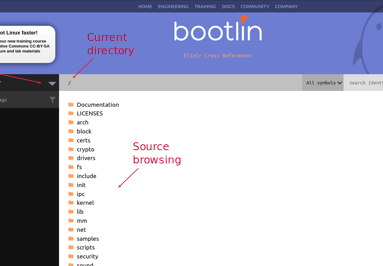
\includegraphics[height=0.8\textheight]{slides/kernel-source-code-management/elixir.pdf}
  \end{center}
\end{frame}

\begin{frame}
  \frametitle{Text editors and IDEs for kernel development}
  \begin{columns}
  \column{0.6\textwidth}
    \begin{itemize}
    \item You can use text editors (Emacs, Vim...) to work on kernel code.
    \item At least Vim and Emacs support ctags and cscope and therefore
          can help with symbol lookup and auto-completion.
    \item It's also possible to use more elaborate IDEs to develop
          kernel code, such as Eclipse, QtCreator and most often
          Visual Studio Code:
          See Michael Opdenacker's presentation ELCE 2020:
          \begin{itemize}
          \item Title: Using Visual Studio Code for Embedded Linux Development
          \item Slides: \url{https://tinyurl.com/y6d8yje7}
          \item Video: \url{https://youtu.be/YGOZIIOWujc}
          \end{itemize}
    \end{itemize}
  \column{0.4\textwidth}
    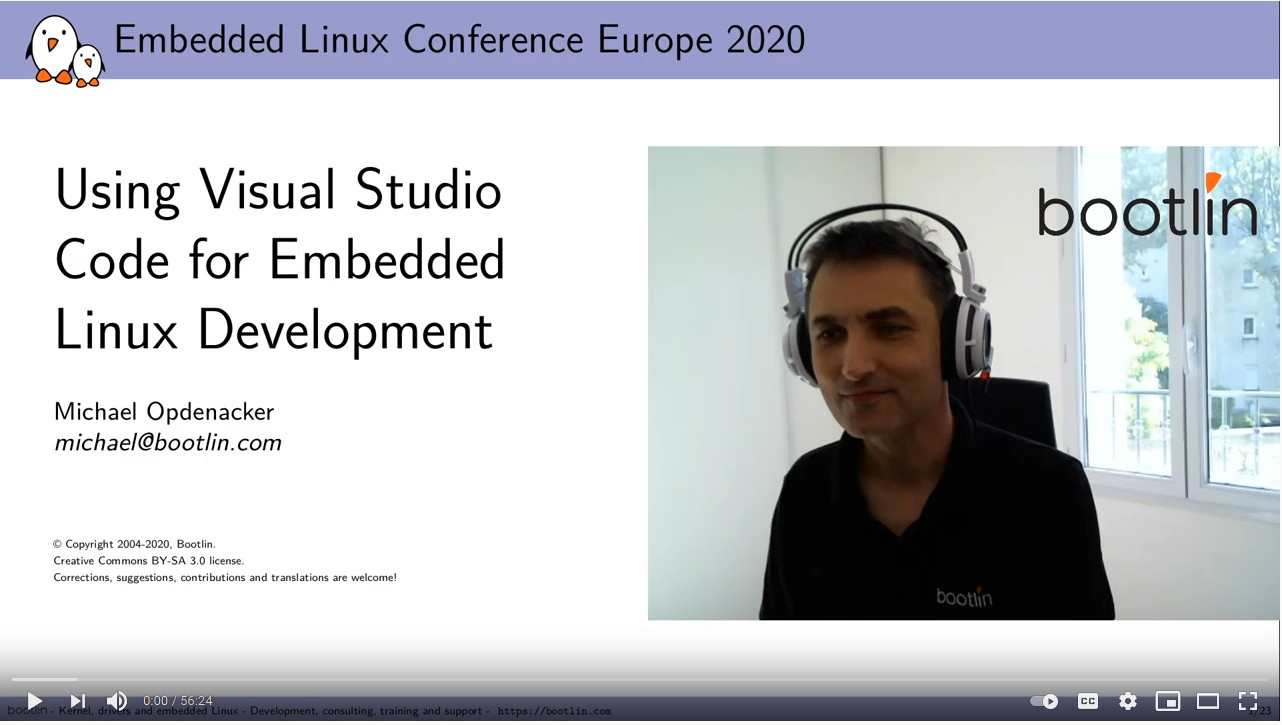
\includegraphics[width=\textwidth]{common/opdenacker-using-vscode.jpg}
  \end{columns}
\end{frame}
